\documentclass[14pt,a4paper,twoside]{article}
\usepackage[top=0.25in]{geometry}
\usepackage{graphicx}
\usepackage{wrapfig}
\usepackage{float}

\begin{document}
	
	\title{TANISH GARG}
		\author{E-5, C.C.Colony, New Delhi-110007 \\ Contact: 09899525271,  E-mail: tanishgarg96@gmail.com}
	\maketitle
	
	\begin{figure}[!h]
		\centering
		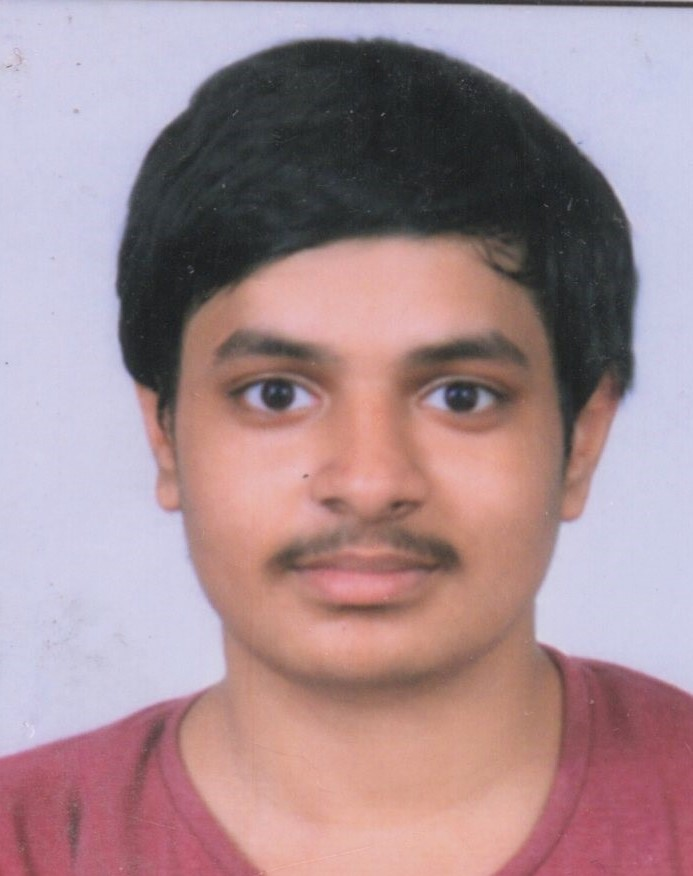
\includegraphics[width=3.5cm,height=3.5cm]{passportpic001}
	\end{figure}		
		
	\section*{\underline{\textbf{Career Objective}}}

	Position as a Robotic engineer and increase my experience and knowledge in field of computers \& electronics
	
	\section*{\underline{\textbf{Education}}}
		\begin{tabular}{|l||c||c||r|}
			\hline
			Standard/Course & School(board)/University & Percentage \\
			\hline
			10th & Guru Harkrishan Public School(CBSE) & 8.4(CGPA)\\
			\hline
			12th & Guru Harkrishan Public School(CBSE) & 80.2\\
			\hline
			B.Tech Electronics & University of Delhi & 78*\\
			
		\end{tabular}
		
		
	  \ * Aggregate percentage till 5th semester	
	\section*{\underline{\textbf{Projects}}}
		\begin{enumerate}
			\item Innovation project: Fan Without Electricity
			\item Innovation project: Problem based learning in Simulation environment
			\item Project at IIT Bombay: Robot Controlling Using ROS 
		\end{enumerate}
	
	\section*{\underline{\textbf{Training and Internship}}}
		\begin{itemize}
			\item Summer Intern at IIT Bombay
		\end{itemize}
		
	\section*{\underline{\textbf{Research Publication}}}
		\begin{enumerate}
			\item Greener Mobile Phones (Co-author)
		\end{enumerate}
	
	\section*{\underline{\textbf{Technical skills}}}
		\begin{itemize}
			\item Computer Languages \& databases
			\begin{itemize}
				\item C/EMBEDDED C		(proficient)
				\item C++				(proficient)
				\item MATLAB			(intermediate, image processing and computer vision)
				\item Python			(intermediate)
				\item JAVA				(intermediate)
				\item MySQL				(intermediate)
				\item XML				(intermediate)
				\item Assembly 			(intermediate)
				\item HTML				(novice)	
			\end{itemize}
		\item Processors/Microcontroller
		\begin{itemize}
			\item ATmega 2560		
			\item ATmaga 16
			\item AT90s2313
			\item Intel 8086					
		\end{itemize}
		\item Robot Operating System(ROS-Indigo) (Intermediate)   
		
		\end{itemize}
		
	\section*{\underline{\textbf{Soft skills}}}
		\begin{enumerate}
			\item Creative \& practical thinking 
			\item Quickly adaptive to new environment
			\item Experienced leadership skills in various department events. 
			
		\end{enumerate}
		
	\section*{\underline{\textbf{Extra Curricular activities}}}
		\begin{itemize}
			\item Enterprenuer (T-SHIRT printing and Selling)
			\item volunteering in department events		
		\end{itemize}
		
	\section*{\underline{\textbf{Co-Curricular activities}}}
		\begin{enumerate}
			\item Robotics
			\item learning softwares like LABView/Multisim
		\end{enumerate}
		
	\section*{\underline{\textbf{Achievements}}}
		\begin{enumerate}
			\item 1st in e-Yantra Robotics Competetion-2015 (Theme: Recyclable Waste Management)
			\item School rank 1st in 15th SOF-National Science olympiad  
			\item 3rd position in delhi region in college level National Anveshika Experimental Skill Test 2015
		\end{enumerate}	
		
	\section*{\underline{\textbf{Hobbies}}}
		\begin{enumerate}
			\item Reading novels(sci-fi,thriller,fantasy,mysteries)
			\item Exploring Computer languages and Webdesigner/Appdesigner websites
		\end{enumerate}
	
		
	\section*{\underline{\textbf{Personal Information}}}
		\begin{enumerate}
			\item Languages known:
				\begin{enumerate}
					\item Hindi
					\item English
					\item Punjabi
				\end{enumerate}
			\item Date Of Birth: 26th-february-1996
			\item Nationality: Indian
			\item Contact details: 09899525271, 011-27457891
			\item E-mail: tanishgarg96@gmail.com
		\end{enumerate}
		
	\section*{\underline{\textbf{Reference}}}

\hspace{12pt} Dr. Praveen Kant Pandey

Professor

Maharaja Agrasen College

University Of Delhi

Tel: 9910158848    
	
	\section*{\underline{\textbf{Declaration}}}
		I hereby declare that the above cited information is true to the best of my knowledge and belief, if given a chance, I can prove myself.
	
	
\end{document}